\documentclass[]{scrartcl}
\usepackage[utf8]{inputenc}
\usepackage{graphicx}
\usepackage{amsmath}
\usepackage{float}

\title{Technik und Technologie vernetzter Systeme  \\ Abgabe der Praktikumsaufgabe 1}

\author{Maria Lüdemann und Birger Kamp}

\begin{document}

\maketitle

\section{Projektschritt 1:Laboreinbindung von Gateways und Sensorknoten}
Nach der Durchführung des Projektschritts 1 anhand des Szenarios 1 haben wir einen Wireshark Mitschnitt gespeichert, der die Unterhaltung der Bestandteile des Netzwerks mitschneidet. Der Mitschnitt ist in Figur \ref{fig:wireshark_1} gezeigt.

\begin{figure}[H]
	\centering
	\includegraphics[width=1\linewidth]{wireshark_1.png}
	\label{fig:wireshark_1}
\end{figure}

Hier zu sehen ist der Ablauf des Neighbor Solicitation Protokolls. Der Ablauf wird im folgenden Flussdiagramm noch einmal verdeutlicht. 


\begin{figure}[H]
	\centering
	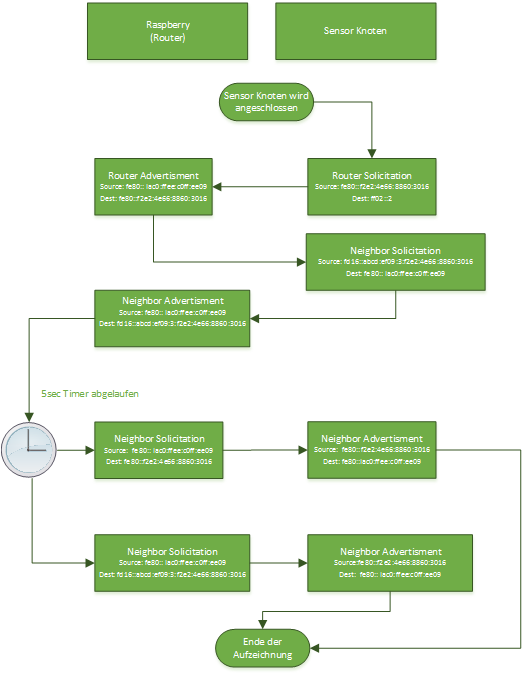
\includegraphics[width=1\linewidth]{flussdiagramm.png}
	\label{fig:flussdiagramm}
\end{figure}

In Diagramm \ref{fig:flussdiagramm} ist zu sehen, dass beim Anschließen des Sensor Knotens, selbiger per \textit{Router Solicitation} nach einem Router fragt. Darauf antwortet der Raspberry Pi und gibt sich als Router bekannt. Daraufhin erfragt der Sensor Knoten mit einer \textit{Neighbor Solicitation} seine Nachbarschaft. Der Raspberry Pi antwortet mit einem \textit{Neighbor Advertisment}. Auffällig ist, dass nach 5 Sekunden der Timer abläuft und die Nachbarschafts Anfragen erneut gesendet werden. Sowohl der Raspberry als auch der Sensor Knoten senden \textit{Neighbour Solicitations} und jeweilige \textit{Advertisements}.\\

\textbf{Auffälligkeit}\\
Nach RFC 6775 (Abschnitt 3.3) sendet der Host eine \textit{Neighbor Solicitation} an den Router mit einer gewissen Lifetime. Sollte die Lifetime ablaufen, dann erneuert der Host diesen Eintrag. Der Router fragt allerdings nicht aktiv nach, ob der Host noch erreichbar ist. Die Anfragen nach dem oben gezeigtem Timeout sollten gemäß RFC 6775 nicht passieren!


\section{Projektschritt 2:RPL Routing im Labornetz}
In Projektschritt 2 haben wir nach Szenario 2 unseren Versuchsaufbau ausgerichtet und durchgeführt. Im gemeinsamen Testlauf wurde durch Wireshark ein Mitschnitt der Kommunikation der Knoten erzeugt. Dieser lief über einige Zeit und umfasst insgesamt mehrere Tausend Nachrichten. In einem weiteren Schritt wurden alle Nachrichten die das RPL Protokoll betreffen analysiert um zu sehen wie es genutzt wird um eine Kommunikation aufzubauen. 

\subsection{Nachrichten und Informationsaustausch}
Die Nachrichten die im Rahmen des RPL Protokolls ausgetauscht werden sind entweder \textit{DODAG Information Object, DODAG Information Solicitation, Destination Advertisment Object (DAO)} oder \textit{Destination Advertisment Object Acknowledgment}. Dadurch werden die Informationen verteilt welche Knoten Teil des Netzwerkes sind und wie die Knoten untereinander verbunden sind. Mithilfe der durch die Nachrichten bekanntgegebenen Struktur kann ein Graph aufgebaut werden, der es ermöglicht Nachrichten im Netz zu verteilen. In der Regel hat jeder Knoten einen Parent-Knoten, an den er seine Nachrichten weiterleitet. Ein Parent weiß dabei nichts von seinen Kindern, bis diese sich bei ihm melden. Der Parent-Knoten erfährt außerdem aus der DAO-Nachricht des Kind-Knoten, welche weiteren Knoten über das Kind erreichbar sind.

Mithilfe der durch das RPL erzeugten Schema können dann Datennachrichten übermittelt werden. Die Knoten wissen wen sie adressieren müssen um Nachrichten zu verteilen. Als erstes ihren Parent der das Datenpaket dann gegebenenfalls weiterleitet. In Figur \ref{fig:RPL_Baum}  ist dies durch den Ping verdeutlicht der an den RPL-Root gehen soll aber vorher über einen anderen Knoten (den Parent-Knoten) weitergeleitet wird.

Aufgrund der Nachrichten und deren Inhalt konnten wir in unserem Versuchsaufbau folgenden Baum entwerfen der sich aus einem ausgewählten Teil unseres Nachrichten Mitschnitts ergibt.

\begin{figure}[H]
	\centering
	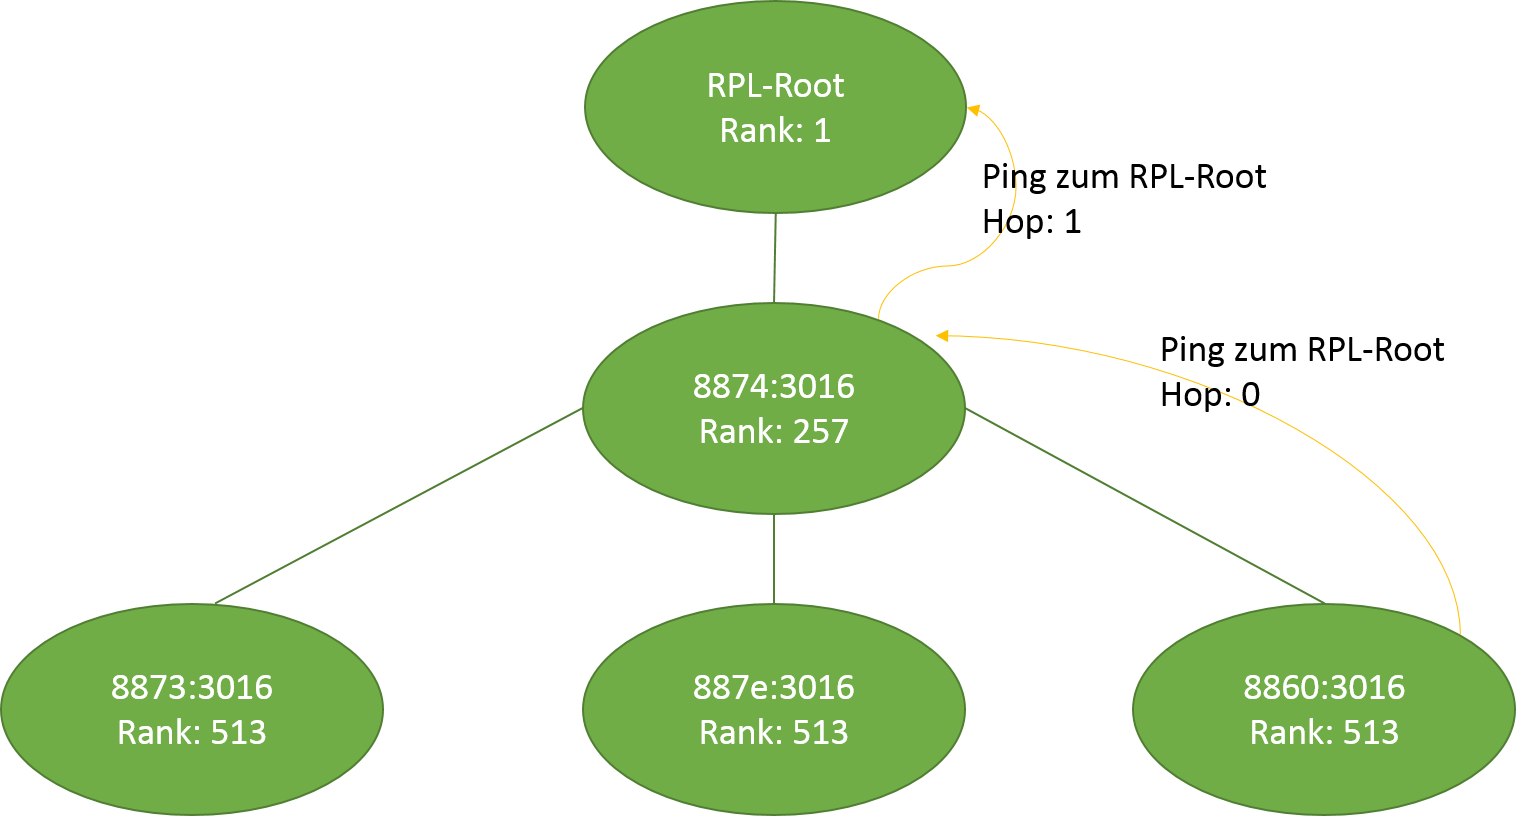
\includegraphics[width=1\linewidth]{RPL_Baum.png}
	\label{fig:RPL_Baum}
\end{figure}


\section{Projektschritt 3: Datenverteilung und Messung}
Der dritte Projektschritt wurde im zweiten Praktikumstermin ausgeführt. Dabei ging es darum die in Projektschritt 1 und 2 bearbeiteten Protokolle zu vergleichen und sie hinsichtlich Zuverlässigkeit und Zeitverhalten zu prüfen. Dafür haben wir sowohl in den zweier Gruppen wie auch in der Praktikumsgruppe selbst Diskussionen und Tests durchgeführt und sind mit unterschiedlichen Ansätzen an die Aufgabenstellung herangegangen.

\subsection{Testaufbau}
Wir entschlossen uns einen einfachen Ping mit verschiedenen Paketgrößen in beiden Szenarien zu versenden um verfolgen zu können wie lange unterschiedlich große Pakete in den Szenarien benötigen sowie wie zuverlässig die Pakete bei steigender Größe ankommen.
Dabei war der Ablauf, dass wir bei einer Ping-Paketgröße von 16 Byte (Der Header den der Ping darauf rechnet nicht mitgezählt) und dann immer verdoppelt haben bis das Paket nicht mehr sein Ziel erreicht. Jeden Ping haben wir 50 Mal ausgeführt und die Ergebnisse gemittelt. Sowohl die Ergebnisse als auch die Erkenntnisse sind in Tabelle \ref{table_ping_result} zu finden.

\subsection{Szenario 2 Ping}

Im zweiten Szenario war es schwierig über für alle Ping-Größen konstante Mess-Werte zu erzeugen da sich je nach Anzahl der aktiven Knoten im Raum die Hop-Anzahl geändert hat. Wir haben uns allerdings Mühe gegeben die Werte möglichst gleichmäßig zu erzeugen. Durch diesen Effekt konnten wir allerdings beobachten das ein zusätzlicher Hop bereits einen Anstieg der Zeit verursachte und auch die Verlustrate steigen lässt.

\begin{table}[H]
\centering
\begin{tabular}{|c|c|c|c|c|c|}
  \hline
  \textbf{Paketgröße} & \textbf{Paketverlust} & \textbf{Zeit (Mittelwert)} & \textbf{Zeit (Min)} & \textbf{Zeit (Min)} & \textbf{Hops} \\
  \hline
   16 & 14\% & 20,33 & 17,72 & 38,37 & 3-4\\
  \hline
   32 & 28\% & 27,296 & 25,086 & 38,171 & 4\\
  \hline
   64 & 44\% & 27,296 & 37,195 & 46,51 & 3\\
  \hline
   128 & 46\% & 55,335 & 49,336 & 79,487 & 3\\
  \hline
   144 & 62\% & 55,743 & 53,212 & 68,738 & 3\\
  \hline
\end{tabular}
	\caption{Ping mit c = 50 Die Paketgröße ist die von uns angegebene Größe ohne Header}
	\label{table_ping_result_scenario2}
\end{table}

Anhand der Daten in Tabelle \ref{table_ping_result} ist zu erkennen, dass die Größe der Pakete stark mit der Zeit in Zusammenhang steht, die die Pakete benötigen. Ebenso steigt der Verlust den die Pakete erleiden. Die Anzahl der Hops ist ebenfalls sehr ausschlaggebend, was die Übertragungsschwindigkeit und -zuverlässigkeit der Pakete betrifft. Werden plötzlich zusätzliche Hops in die Paket-Route geschaltet oder entfernt, beeinflusst das die Zuverlässigkeit der Übertragung stark.

Ab einer Paketgröße von 144 Byte ist keiner der Pings mehr übertragen worden bzw. wir haben keine Ping-Reply vom Ping-Empfänger erhalten, die Verlustrate steigt dort auf ca. 100 Prozent. Das führen wir darauf zurück, dass ab einer gewissen Größe Ping-Pakete in mehrere TCP-Pakete geteilt werden. Von diesen Paketen müssen allerdings alle beim Empfänger ankommen um einen erfolgreichen Ping zu gewährleisten. Ab der Größe von 145 Byte sind dies aber so viele TCP-Pakete, dass in der Regel kein Paket sein Ziel erreicht und wir keine erfolgreichen Pings mehr verzeichnen konnten. Dies ist auch ein Hinweis darauf, das eine zuverlässige Übertragung der Daten über dieses Protokoll nicht möglich ist.


\subsection{Szenario 1 Ping}

Im zweiten Versuch haben wir das Szenario 1 aufgebaut und den Test im gleichen Maße wie schon in Szenario 2 durchgeführt. Hier hatten wir allerdings schnell das Problem, dass der Sensor-Knoten die IPv6-Adresse verliert. Dies ist ein Problem auf das wir keinen Einfluss hatten und mit dem Protokoll nichts zu tun hat. Um das Problem zu umgehen haben wir in diesem Durchlauf die Ping Anzahl auf 10 verringert da es nicht möglich war 50 Pings an einem Stück durchzuführen.

Das Ergebnis der Messung ist in Tabelle \ref{table_ping_result_scenario1} aufgeführt

\begin{table}[H]
\centering
\begin{tabular}{|c|c|c|c|c|c|}
  \hline
  \textbf{Paketgröße} & \textbf{Paketverlust} & \textbf{Zeit (Mittelwert)} & \textbf{Zeit (Min)} & \textbf{Zeit (Min)} \\
  \hline
   16 & 6\% & 10,387 & 8,549 & 18,955\\
  \hline
   32 & 16\% & 11,384 & 9,65 & 20,537\\
  \hline
   64 & 0\% & 17,587 & 17,058 & 20,895\\
  \hline
   128 & 15\% & 22,048 & 20,602 & 23,167\\
  \hline
   144 & 5\% & 23,189 & 22,356 & 24,32\\
  \hline
\end{tabular}
	\caption{Die Paketgröße ist die von uns angegebene Größe ohne Header Hopanzahl Konstant 2}
	\label{table_ping_result_scenario1}
\end{table}

Aufgrund des Aufbaus passieren die Ping-Pakete in diesem Szenario konstant zwei Hops. eine kabelgebundene Verbindung zwischen Arbeitsrechner und Raspberry Pi und eine kabellose Verbindung vom Raspberry Pi zum Sensor-Knoten. Auffällig auch hier ist die mit der Größe steigende Übertragungszeit. Eher ungewöhnlich wirkt hier der Paketverlust den wir aber auf die Probleme mit dem Sensorknoten und einem zu dem Zeitpunkt stark schwankendem Funkverkehr im Praktikumsraum zurückführen. Überraschend war hier die erst gering wirkende Verlustrate von 5 Prozent im letzten Mess-Schritt, doch bei Vergrößerung der Paketgröße über 144 Byte hinaus ist es auch hier nicht mehr möglich einen Ping erfolgreich durchzuführen.


\subsection{Vergleich und weitere Beobachtungen}

Im Vergleich der beiden Messungen tritt stark hervor, dass sowohl in Zeit wie auch Verlust die Übertragung über das Kabel privilegiert ist. Der Funkverkehr, vor allem über eine steigende Anzahl an Hops führt zu hohen Latenzen und hohen Verlustraten. Allerdings hatten wir den Eindruck, dass Szenario 1 deutlich anfälliger für den Funkverkehr im Raum ist als das Szenario 2.

Eine Beobachtung die wir machen konnten war, dass am Anfang eines Pings, besonders wenn wir den Sensorknoten gerade Neustarten mussten, deutlich zu merken war dass der Sensorknoten eine Zeit braucht, um sich im Netzwerk wieder einzurichten. Ebenso war es sehr auffällig, dass der Verkehr im Raum großen Einfluss hatten. Der Gruppe ganz hinten im Raum war es über die meiste Zeit praktisch unmöglich zu pingen, bis zu dem Zeitpunkt wo die meisten aufgehört haben zu senden. Anhand unserer Pingverluste und der Umfrage an die anderen Gruppen konnten wir feststellen, dass sobald auch andere Gruppen gesendet haben, unsere Verluste dramatisch steigen bis zu einem Maße, dass wir gar nichts mehr empfangen haben. Dieses Problem stellte sich bei uns vor allem in Szenario 1 heraus, bei anderen Gruppen aber auch im Szenario 2.


\end{document}